% document formatting
\documentclass[10pt]{article}
\usepackage[utf8]{inputenc}
\usepackage[left=1in,right=1in,top=1in,bottom=1in]{geometry}
\usepackage[T1]{fontenc}
\usepackage{xcolor}

% math symbols, etc.
\usepackage{amsmath, amsfonts, amssymb, amsthm}

% lists
\usepackage{enumerate}

% images
\usepackage{graphicx} % for images
\usepackage{multirow}

% code blocks
\usepackage{minted, listings} 

% verbatim greek
\usepackage{alphabeta}

\graphicspath{{./assets/images}}

\newcommand{\solution}{\textbf{Solution:}} 
\newcommand{\example}{\textbf{Example: }}
\newcommand{\sinc}{\text{sinc}}

\title{EC ENGR 102 Week 5}

\author{Aidan Jan}
\date{\today}

\begin{document}
\maketitle

\subsection*{Sawtooth Signal}
The sawtooth signal is given by $f(t) = t \mod 1$.  It is plotted below:
\begin{center}
    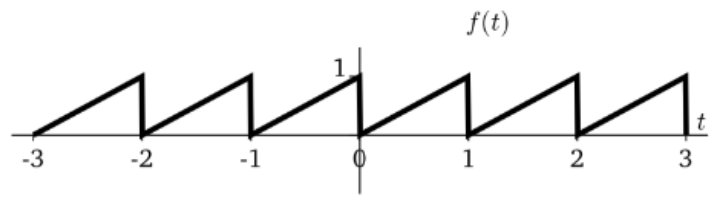
\includegraphics[scale=0.9]{W4_13.png}
\end{center}
This signal has a period of $T_0 = 1$.  Now, when $k = 0$,
\begin{align*}
    c_0 &= \int_0^1 te^0 \text{d}t\\
    &= \left.\frac{t^2}{2}\right|_0^1\\
    &= \frac{1}{2}
\end{align*}
This is also the Fourier series of the time-limited signal $f(t) = t$ on the interval $[0, 1)$.  The time-limited signal can be made periodic via a periodic extension.

\subsection*{Fourier Series Properties}
There are interesting symmetries and properties of the Fourier series that are worth expanding upon.
\begin{itemize}
    \item $c_0$ \textbf{is the average of the signal}.  Not that for $k = 0$, we have that
    \[c_0 = \frac{1}{T_0} \int_{t_0}^{t_0 + T_0} f(t) \text{d}t\]
    Thus, $c_0$ is exactly the time-averaged mean of the signal and corresponds to a constant value (i.e., it has no sinusoidal component).  For this reason, it is sometimes called the "DC component."  DC stands for direct current in circuits, and refers to non-alternating (sinusoidal) currents.  The DC component is the average value taken on by a signal.
\end{itemize}

\subsection*{Fourier Symmetry}
We can apply Euler's formula to re-write the Fourier coefficients, and reveal some symmetries:
\begin{align*}
    c_k &= \frac{1}{T_0} \int_{t_0}^{t_0 + T_0} f(t) e^{-j\frac{2\pi kt}{T_0}}\text{d}t\\
    &= \frac{1}{T_0} \int_{t_0}^{t_0 + T_0} f(t) \left[\cos\left(\frac{2\pi k}{T_0}t\right) - j \sin\left(\frac{2\pi k}{T_0}t\right)\right]\text{d}t\\    &= \frac{1}{T_0} \int_{t_0}^{t_0 + T_0} f(t) \cos\left(\frac{2\pi k}{T_0}t\right) \text{d}t - \frac{j}{T_0} \int_{t_0}^{t_0 + T_0} f(t) \sin\left(\frac{2\pi k}{T_0}t\right)\text{d}t
\end{align*}
In the above equation, the left term is the real part, the right term is the imaginary part.\\\\
If $f(t)$ is real, then so are:
\begin{align*}
    \mathfrak{R}(c_k) &= \frac{1}{T_0}\int_{t_0}^{t_0 + T_0}f(t)\cos\left(\frac{2\pi k}{T_0}t\right)\text{d}t\\
    \mathfrak{I}(c_k) &= -\frac{1}{T_0}\int_{t_0}^{t_0 + T_0}f(t)\sin\left(\frac{2\pi k}{T_0}t\right)\text{d}t
\end{align*}
Therefore, for $f(t)$ real, and using the fact that $\cos(k)$ is even and $\sin(k)$ is odd, we have the following symmetries:
\begin{align}
    \mathfrak{R}(c_k) &= \mathfrak{R}(c_{-k})\\
    \mathfrak{I}(c_k) &= \mathfrak{I}(c_{-k})\\
    c_k^* &= c_{-k}\\
    |c_k| &= |c_{-k}|\\
    \angle c_k &= -\angle c_k^*\\
    c_k &= c_{-k}\hspace{1cm} \text{(only if $x(t)$ is even)}\\
    c_k &= -c_{-k}\hspace{1cm} \text{(only if $x(t)$ is odd)}
\end{align}
\subsubsection*{Proof of (1)}
\begin{align*}
    \mathfrak{R}(c_{-k}) &= \frac{1}{T_0} \int_{t_0}^{t_0 + T_0}f(t) \cdot \cos\left(-\frac{2\pi k}{T_0} t\right) \text{d}t\\
    &= \frac{1}{T_0} \int_{t_0}^{t_0 + T_0}f(t) \cdot \cos\left(\frac{2\pi k}{T_0} t\right) \text{d}t\\
    &= \mathfrak{R}(c_{-k})
\end{align*}
\subsubsection*{Proof of (2)}
\begin{align*}
    \mathfrak{I}(c_{-k}) &= -\frac{1}{T_0} \int_{t_0}^{t_0 + T_0}f(t) \cdot \sin\left(-\frac{2\pi k}{T_0} t\right) \text{d}t\\
    &= \frac{1}{T_0} \int_{t_0}^{t_0 + T_0}f(t) \cdot \sin\left(\frac{2\pi k}{T_0} t\right) \text{d}t\\
    &= \mathfrak{I}(c_{-k})
\end{align*}
\subsubsection*{Proof of (3)}
\begin{align*}
    c_k &= \mathfrak{R}(c_k) + j \cdot \mathfrak{I}(c_k)\\
    c_k^* &- \mathfrak{R}(c_k) - j \cdot \mathfrak{I}(c_k)\\
    &= \mathfrak{R}(c_-k) + j \cdot \mathfrak{I}(c_-k)\\
    &= c_{-k}
\end{align*}
\subsubsection*{Proof of (4)}
\begin{align*}
    |c_k| &= \sqrt{\mathfrak{R}^2(c_k) + \mathfrak{I}^2(c_k)}\\
    |c_{-k}| &= \sqrt{\mathfrak{R}^2(c_k) + \mathfrak{I}^2(c_{-k})}\\
    &= \sqrt{\mathfrak{R}^2(c_k) + (-\mathfrak{I}(c_k))^2}\\
    &= |c_k|
\end{align*}
\subsubsection*{Proof of (5)}
\begin{align*}
    \angle c_k &= \arctan \left(\frac{\mathfrak{R}(c_k)}{\mathfrak{I}(c_k)}\right)\\
    &= \arctan \left(\frac{\mathfrak{R}(c_{-k})}{\mathfrak{I}(c_{-k})}\right)\\
    &= \arctan \left(\frac{\mathfrak{R}(c_{k})}{-\mathfrak{I}(c_k)}\right)\\
    &= \angle c_{-k}
\end{align*}
\subsubsection*{Proof of (6)}
\begin{align*}
    c_k &= \frac{1}{T_0} \int_{0}^{T_0} x(t) e^{-jk\omega_0 t} \text{d}t\\
    c_{-k} &= \frac{1}{T_0} \int_{0}^{T_0} x(t) e^{jk\omega_0 t}\text{d}t\\
    \intertext{Let $u = -t$.}
    &= -\frac{1}{T_0} \int_{0}^{-T_0} x(-u) \cdot e^{-jk\omega_0 u} \text{d}u\\
    &= \frac{1}{T_0} \int_{-T_0}^0 x(u) \cdot e^{-jk\omega_0 u} \text{d}u\\
    &= c_k
\end{align*}
\subsection*{Fourier Series Properties}
\begin{itemize}
    \item If $x(t)$ is even, then $x(t) = x(-t)$, and therefore, $c_k = c_{-k}$.  You can see this by realizing that $kt$ only appears in the complex exponential, and therefore negating $t$ has the same effect as negating $k$.
    \[x(t) \text{ even} \Longrightarrow c_k = c_{-k}\]
    \item If $x(t)$ is odd, then $x(t) = -x(-t)$, and therefore, $c_k = -c_{-k}$.  This holds for the same reason as for the even case.
    \[x(t) \text{ odd} \Longrightarrow c_k = -c_{-k}\]
    \item Combining facts, we have that if $x(t)$ is even and real, then $c_k = c_{-k}$ and $c_{-k} = c_k^*$, and so $c_k = c_k^*$.  This means that $c_k$ must be real.
    \[x(t) \text{ even and real} \Longrightarrow c_k \text{ real}\]
    \item If $x(t)$ is odd and real, then $c_k = -c_{-k}$, and because $c_{-k} = c_k^*$, then $c_k = -c_k^*$.  This means that $c_k$ must be imaginary.
    \[x(t) \text{ odd and real} \Longrightarrow c_k \text{ imaginary}\]
\end{itemize}

\subsection*{Perseval's Theorem}
Suppose we want to find the power of a complex signal:
\[\frac{1}{T_0} \int_{t_0}^{t_0 + T_0} |x(t)|^2 \text{ d}t\]
Since $x(t)$ is complex, we split the square to $x(t) \cdot x(t)^*$.  Therefore,
\begin{align*}
    &= \frac{1}{T_0} \int_{t_0}^{t_0 + T_0} x(t) x(t)^* \text{d}t\\
    &= \frac{1}{T_0} \int_{t_0}^{t_0 + T_0} \left[\sum_{k=-\infty}^\infty c_k e^{jk\omega_0 t}\right] \left[\sum_{n=-\infty}^\infty c_n^* e^{-jn\omega_0 t}\right] \text{d}t
    \intertext{We can then switch the order of the summation and integral.}
    &= \frac{1}{T_0} \sum_{k = -\infty}^\infty c_k \sum_{k = -\infty}^\infty c_n^* \cdot \int_{t_0}^{t_0 + T_0} e^{j(k-n)\omega_0 t} \text{d}t\\
    \intertext{Notice that the integral returns $0$ when $k \neq n$, and $T_0$ when $k = n$.  This is because if you expand the exponential using Euler's formula, then you are integrating a cosine and sin over one period, the periods of which will cancel out.  Therefore,}
    &= \frac{1}{T_0} \sum_{-\infty}^\infty c_k \cdot c_k^* \cdot T_0\\
    &= \sum_{k=-\infty}^\infty |c_k|^2
\end{align*}

\textbf{Everything before this point is fair game on Midterm 1.}\\

\section*{Aperiodic Signals}
\begin{itemize}
    \item The Fourier series can model (almost) any \textbf{periodic} or \textbf{time-limited} function as a sum of complex exponentials.  However, most signals we encounter are not necessarily periodic or time-limited.
    \item The \textbf{Fourier transform} allows us to calculate the spectrum of aperiodic signals.
\end{itemize}

\subsection*{Intuition of going from Fourier series to Fourier transform}
Extending Fourier series to the Fourier transform is fairly intuitive.\\\\
The idea is the following:
\begin{itemize}
    \item We can calculate the Fourier series of a periodic or time-limited signal, over some interval of length $T_0$.
    \item A signal that is not periodic can be viewed as a periodic signal, where $T_0$ is infinite.  As $T_0$ is infinite, it never repeats.
    \item But the point is that we can replace our Fourier series calculation as, instead of being over a finite period, $T_0$, being over all time, from $t = -\infty$ to $\infty$.
    \item Mathematically, we can calculate the Fourier series of $f(t)$ over the interval $[-T/2. T/2)$ via:
    \[f(t) = \sum_{k = -\infty}^\infty c_k e^{jk\omega_0 t}\]
    with 
    \[c_k = \frac{1}{T} \int_{-T/2}^{T/2} f(t) e^{-jk\omega-0}\text{d}t\]
    where $\omega_0 = 2\pi/T$.  In the Fourier transform, we're now going to let $T \rightarrow \infty$.
\end{itemize}
\example\\
This is the rect() function.
\begin{center}
    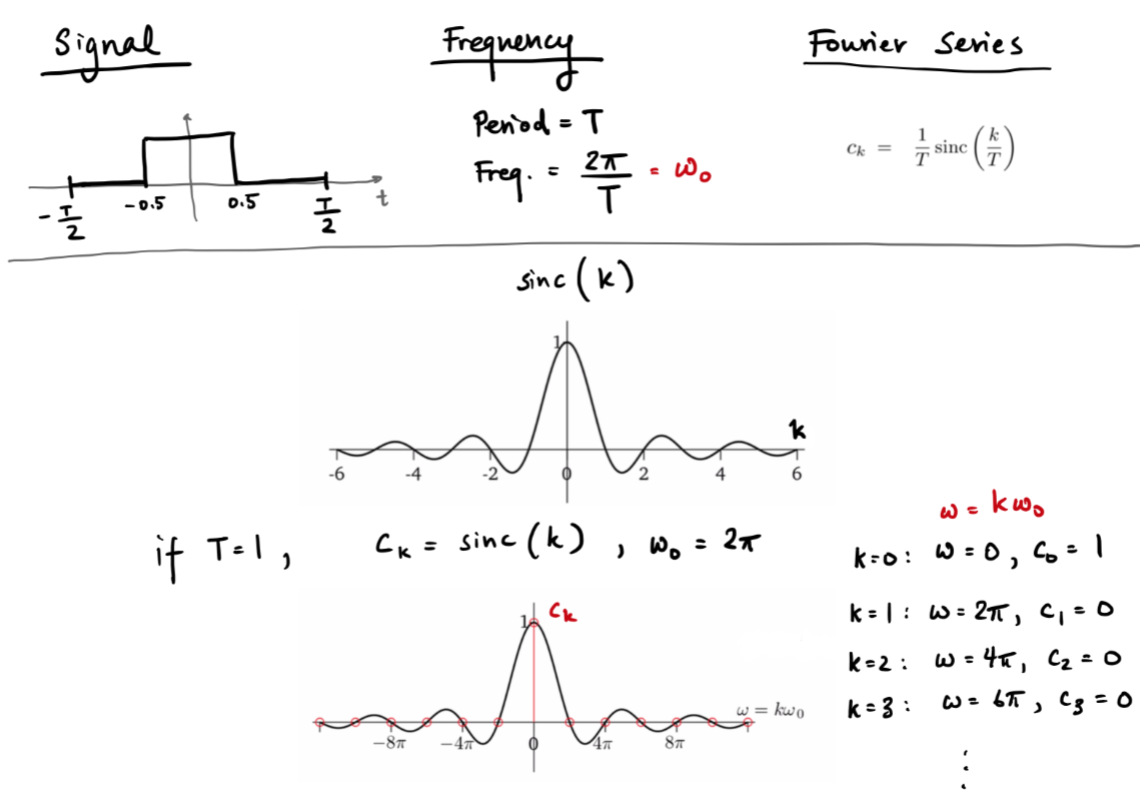
\includegraphics[scale=0.65]{W5_1.png}
\end{center}
\subsection*{Arriving at the Fourier transform}
When $T \rightarrow \infty$, $c_k \rightarrow 0$.
\[c_k = \frac{1}{T} \int_{-\frac{T}{2}}^{\frac{T}{2}} f(t) e^{jk\omega_0 t} \text{d}t\]
To prevent this, we introduce the truncated Fourier transform.
\begin{align*}
    &F_T(j\omega) = \int_{-\frac{T}{2}}^{\frac{T}{2}} f(t) e^{-j\omega t} \text{d}t\\
    \Rightarrow \hspace{0.5cm} & F_T(jk\omega_0) = T \cdot c_k
\end{align*}
Remember that we replace $k\omega_0$ with $\omega$.
\begin{center}
    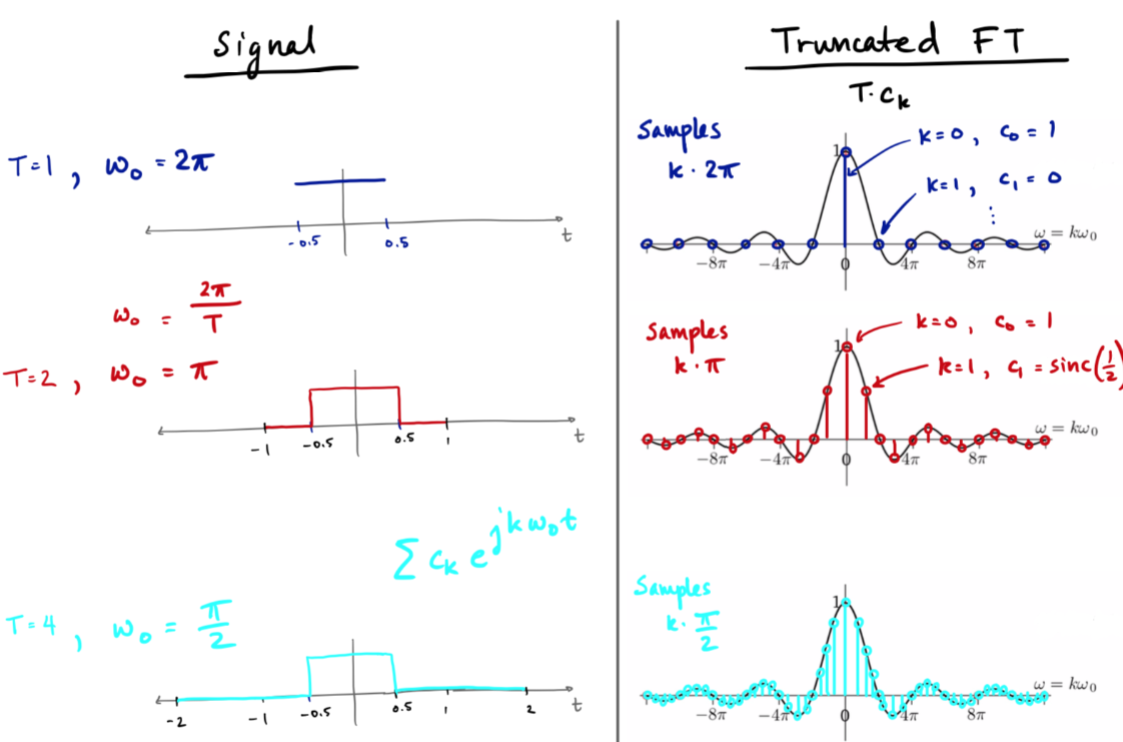
\includegraphics[scale=0.68]{W5_2.png}
\end{center}
The intuition: as $T \rightarrow \infty$, we more finely sample the truncated fourier transform.  $k\omega_0 \rightarrow \omega$, since $\omega_0 \rightarrow 0$ as $T \rightarrow \infty$.\\\\
Now, let's set $T \rightarrow \infty$.  If we do this, then $\omega_0 = 2\pi / T$ will approach 0.  So suppose instead that we define a continuous variable,
\[\omega = \frac{2\pi k}{T}\]
which means that $k$ increases with $T$, so that $\omega = k\omega_0$ is fixed.\\\\
The Fourier transform is the limit of the truncated Fourier transform.
\begin{align*}
    F(k\omega) &= \lim_{T \rightarrow \infty} F_T(j\omega)\\
    &= \lim_{T \rightarrow \infty} \int_{-T/2}^{T/2} f(t) = e^{-j\omega t} \text{d}t\\
    &= \int_{-\infty}^\infty f(t) e^{-j\omega t} \text{d}t
\end{align*}
This is the Fourier transform, which takes you from the time domain, $f(t)$, to the frequency domain, $F(j\omega)$.
\subsubsection*{Fourier Transform Formula}
\[F(j\omega) = \int_{-\infty}^\infty f(t) e^{-j\omega t} \text{d}t\]
\subsection*{Inverting the Fourier Transform}
How do we go from $F(j\omega)$ back to $f(t)$?.  Let's begin by writing the Fourier series.
\begin{align*}
    f(t) &= \lim_{T \rightarrow \infty} f_T(t)\\
    &= \lim_{T \rightarrow \infty} \sum_{k = -\infty}^\infty \frac{1}{T} F_T(jk\omega_0)e^{jk\omega_0 t}
\end{align*}
Now as $T \rightarrow \infty$, what we see is that this approaches an integral.  This is an infinite sum, where the integration "widths" are the infinitesimal $1/T$ and the "heights" are $F_T(jk\omega_0)e^{jk\omega_0 t}$.  To make this more clear, we denote $\Delta \omega = 2\pi / T$, and note that $\omega = k\Delta \omega$.  Then, this sum becomes
\begin{align*}
    f(t) &= \lim_{\Delta \omega \rightarrow 0} \sum_{k = -\infty}^\infty F_T(jk\Delta \omega) e^{jk\Delta \omega t} \frac{\Delta \omega}{2\pi}\\
    &= \frac{1}{2\pi} \int_{-\infty}^\infty F(j\omega) e^{j\omega t} \text{d}\omega
\end{align*}
This is the inverse Fourier transform, which takes you from the frequency domain, $F(j\omega)$ to the time domain, $f(t)$.
\subsection*{Fourier Transform Summary}
The fourier transform is:
\[\boxed{F(j\omega) = \int_{-\infty}^\infty f(t) e^{-j\omega t} \text{d}t}\]
The inverse fourier transform is:
\[\boxed{f(t) = \frac{1}{2\pi} \int_{-\infty}^{\infty} F(j\omega)e^{j\omega t} \text{d}\omega}\]
A few notes:
\begin{itemize}
    \item Like in Fourier series, the inversion formula for $f(t)$ is accurate when $f(t)$ is continuous, but produces the midpoint when $f(t)$ has jumps.
    \item These two are almost identical in form, except for the sign of the complex exponential and the factor of $1/2\pi$.
    \item Check your intuition when you look at these formulas: to go from the time domain to frequency domain (Fourier transform) you should integrate away time (giving a function of frequency).  Likewise, to go from the frequency domain to the time domain (inverse Fourier transform) you should integrate away frequency (giving a function of time).
\end{itemize}

\subsection*{A sufficient condition for the existence of the Fourier transform}
    \begin{itemize}
        \item From $F(j\omega)$, we can determine $f(t)$ and vice versa (if it's well-behaved; e.g., at discontinuities, the Fourier transform will return the midpoint).
        \item Not every function has a Fourier transform.  For example, a sufficient condition for a Fourier transform is that it should have finite energy.  Note,
        \begin{align*}
            |F(j\omega)| &= \left|\int_{-\infty}^\infty f(t) e^{-j\omega t} \text{d}t\right|\\
            &\leq \int_{-\infty}^\infty \left| f(t) e^{-j\omega t} \right| \text{d}t\\
            &= \int_{-\infty}^\infty|f(t)| \text{d}t\\
            &< \infty
        \end{align*}
        \item The above is a sufficient (but not necessary) requirement for the existence of the Fourier transform.
    \end{itemize}

\subsection*{Example: Fourier Transform of rect()}
\begin{align*}
    F(j\omega) &= \int_{-\infty}^\infty \text{rect}(t/T) e^{-j\omega t} \text{d}t\\
    &= \int_{-T/2}^{T/2} e^{-j\omega t} \text{d}t\\
    &= \left.\frac{e^{-j\omega t}}{-j\omega}\right|_{-T/2}^{T/2}\\
    &= \frac{1}{-j\omega} \left(e^{-j\omega T/2} - e^{jwT/2}\right)\\
    &= \frac{1}{-j\omega}(-2j \sin(\omega T/2))\\
    &= \frac{2\sin(\omega T/2)}{\omega}\\
    &= \frac{T \sin(\pi(\omega T/2\pi))}{\pi(\omega T/2\pi)}\\
    &= T \sinc(\omega T / 2\pi)
\end{align*}
Note that here, we went through some extra algebra to get things into the $\sinc(\cdot)$ form.  This is out of convenience.  Thus, we have that
\[\text{rect}(t/T) \Longleftrightarrow T \sinc(\omega T/2\pi)\]

\subsection*{Example: Fourier Transform of a Causal Exponential}
Let's find the Fourier transform of
\[f(t) = \begin{cases}e^{-at} & t \geq 0 \\ 0 & \text{otherwise}\end{cases}\]
for $a > 0$.\\\\
Its Fourier transform is 
\begin{align*}
    F(j\omega) &= \int_{-\infty}^\infty e^{-at} u(t) e^{-j\omega t} \text{d}t\\
    &= \int_0^\infty e^{-at} \cdot e^{-j\omega t} \text{d}t\\
    &= \int_0^\infty e^{-(a + j\omega)t} \text{d}t\\
    &= \left.-\frac{1}{a + j\omega} e^{-(a = j\omega) \cdot t}\right|_{t = 0}^{t = \infty}\\
    &= \frac{1}{a + j\omega}
\end{align*}
\[e^{at}u(t) \Longleftrightarrow \frac{1}{a + j\omega}\]

Below is the spectrum of the causal exponential for $a = 1$.
\begin{center}
    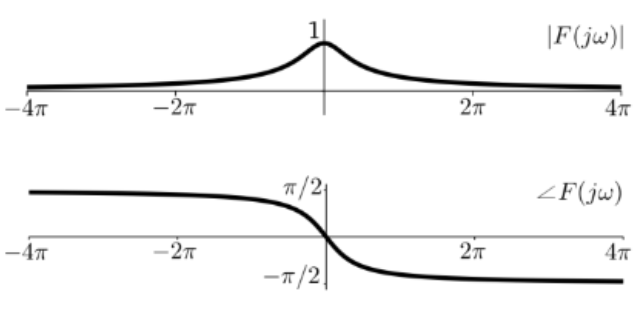
\includegraphics[scale=0.8]{W5_3.png}
\end{center}

\subsubsection*{Fourier Transforms we know}
\begin{align*}
    \text{rect}(t/T) &\Longleftrightarrow T \sinc(\omega T / 2\pi)\\
    e^{-at} u(t) &\Longleftrightarrow \frac{1}{a + j\omega}
\end{align*}

\subsection*{Fourier Symmetries}
Derivations analogous to Fourier series
\begin{itemize}
    \item For any $f(t)$, whether it be real, imaginary, or complex:
    \begin{itemize}
        \item $f(t)$ even $\rightarrow F(j\omega)$ even.
        \item $f(t)$ odd $\rightarrow F(j\omega)$ odd.
    \end{itemize}
    \item A \textit{real} signal has a Hermitian Fourier transform:
    \[F(-j\omega) = F^*(j\omega)\]
    \item An \textit{imaginary} signal has an anti-Hermitian Fourier transform:
    \[F(-j\omega) = -F^*(j\omega)\]
    \item Furthermore,
    \begin{itemize}
        \item For $f(t)$ real and even, $F(j\omega)$ is real and even.
        \item For $f(t)$ real and odd, $F(j\omega)$ is imaginary and odd.
        \item For $f(t)$ imaginary and odd, $F(j\omega)$ is real and odd.
        \item For $f(t)$ imaginary and even, $F(j\omega)$ is imaginary and even.
    \end{itemize}
\end{itemize}

\section*{The Fourier Transform Operator}
To denote the operation of taking the Fourier transform, we use $\mathcal{F}(\cdot)$ or $\mathcal{F}[\cdot]$.  That is, if
\[f(t) \Longleftrightarrow F(j\omega)\]
we may alternately write this as
\[F(j\omega) = \mathcal{F}[f(t)]\]
Likewise, the operator $\mathcal{F}^{-1}$ refers to the inverse Fourier transform.  Therefore, 
\[\mathcal{F}^{-1}[F(j\omega)] = f(t)\]
This also means that
\[\mathcal{F}^{-1}[\mathcal{F}[f(t)]] = f(t)\]
at all points of continuity in $f(t)$.

\subsection*{Summary of all properties of Fourier Transform (can be used without proof)}
\begin{enumerate}
    \item \textbf{Linearity:}
    \[\boxed{\mathcal{F}[a f_1(t) + b f_2(t)] = a \mathcal{F}[]f_1(t) + b\mathcal{F}[f_2(t)]}\]
    \item \textbf{Time scaling:}
    \[\boxed{\mathcal{F}[f(at)] = \frac{1}{|a|}F\left(j\frac{\omega}{a}\right)}\]
    \item \textbf{Time reversal:}
    \[\boxed{\mathcal{F}[f(-t)] = F(-j\omega)}\]
    \item \textbf{Complex conjugate:}
    \[\boxed{f^*(t) \Longleftrightarrow F^*(-j\omega)}\]
    \item \textbf{Duality:}
    \[\boxed{F(t) \Longleftrightarrow 2\pi f(-j\omega)}\]
    \item \textbf{Time-shifting:}
    \[\boxed{\mathcal{F}[f(t - \tau)] = e^{-j\omega \tau} F(j\omega)}\]
    \item \textbf{Derivative:}
    \[\boxed{\mathcal{F}[f'(t)] = j\omega F(j\omega)} \]
    \item \textbf{Convolution:}
    \[\boxed{\mathcal{F}[(f_1 * f_2)(t)] = F_1(j\omega) F_2(j\omega)}\]
    \item \textbf{Perseval's Theorem:}
    \[\boxed{\int_{-\infty}^\infty |f(t)|^2 \text{d}t = \frac{1}{2\pi} \int_{-\infty}^\infty |F(j\omega)|^2 \text{d}\omega}\]
    \item \textbf{Multiplication:}
    \[\boxed{\mathcal{F}[f_1(t)f_2(t)] = \frac{1}{2\pi} (F_1 * F_2)(j\omega)}\]
    \item \textbf{Modulation:}
    \[\boxed{\mathcal{F}[f(t) e^{j\omega_0 t}] = F(j(\omega - \omega_0))}\]
\end{enumerate}

\subsection*{Proof of Linearity}
For two signals, $f_1(t)$ and $f_2(t)$ and two complex numbers $a$ and $b$,
\[\boxed{\mathcal{F}[a f_1(t) + b f_2(t)] = a \mathcal{F}[]f_1(t) + b\mathcal{F}[f_2(t)]}\]
Another way to write this is
\[a f_1(t) + b f_2(t) \Longleftrightarrow aF_1(j\omega) + bF_2(j\omega)\]
where $F_1(j\omega) = \mathcal{F}[f_1(t)]$ and $F_2(j\omega) = \mathcal{F}[f_2(t)]$.\\\\
To show this, note:
\begin{align*}
    \mathcal{F}(af_1(t) + bf_2(t)) &= \int_{-\infty}^\infty (af_1(t) + bf_2(t))e^{-j\omega t} \text{d}t\\
    &= \int_{-\infty}^\infty af_1(t) e^{-j\omega t} \text{d}t + \int_{-\infty}^\infty bf_2(t) e^{-j\omega t} \text{d}t\\
    &= a\mathcal{F}[f_1(t)] + b\mathcal{F}[f_2(t)]
\end{align*}
This extends to finite combinations, i.e., 
\[\mathcal{F}\left[\sum_{k = 1}^K a_k f_k(t)\right] = \sum_{k = 1}^K a_k \mathcal{F}[f_k(t)]\]

\subsection*{Linearity example}
Consider the signal:
\[f(t) = \begin{cases}\frac{1}{2} & \frac{1}{2} \leq |t| \leq 1 \\ 1 & |t| \geq \frac{1}{2}\end{cases}\]
This signal steps up and then steps down, as shown below.
\begin{center}
    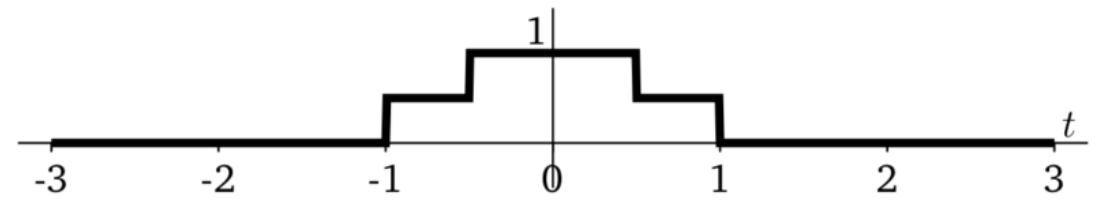
\includegraphics[scale=0.7]{W5_4.png}
\end{center}
\[f(t) = \frac{1}{2} \text{rect}\left(\frac{t}{2}\right) + \frac{1}{2} \text{rect}(t)\]
\[\text{rect}\left(\frac{t}{T}\right)\Longleftrightarrow T \sinc \left(\frac{\omega T}{2\pi}\right)\]
and therefore,
\begin{align*}
    F(j\omega) &= \frac{1}{2}2\sinc(2\omega/2\pi) + \frac{1}{2} \sinc(\omega/2\pi)\\
    &= \sinc(\omega/\pi) + \frac{1}{2} \sinc(\omega/2\pi)
\end{align*}
This is shown below:
\begin{center}
    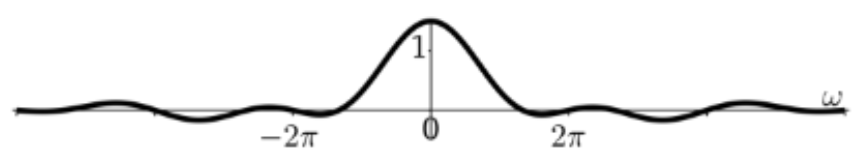
\includegraphics[scale=0.7]{W5_5.png}
\end{center}

\subsection*{Proof of Time-scaling Property}
If $\mathcal{F}[f(t)] = F(j\omega)$, then
\[\boxed{\mathcal{F}[f(at)] = \frac{1}{|a|}F\left(j \frac{\omega}{a}\right)}\] 
Note, for real $a$:
\begin{itemize}
    \item If $a > 1$, $f(t)$ contracts, but its Fourier transform expands.
    \item If $0 < a < 1$, then $f(t)$ expands, but its Fourier transform contracts.
    \item Thus, stretching a signal in time compresses its Fourier transform, and compacting the signal expands its Fourier transform.
\end{itemize}
To show this, let's consider $a > 0$.  (The proof is essentially the same for $a  0$)  We will use a variable change, $\tau = at$, which means that $\text{d}\tau = a\text{d}t$.
\[\mathcal{F}(f(at)) = \int_{-\infty}^\infty f(at) e^{-j\omega t} \text{d}t\]
\example\\
Knowing that
\[\text{rect}(t/T) \Longleftrightarrow T\sinc(\omega T/2\pi)\]
we can then determine that the Fourier transform of $\text{rect}(t)$ is $\sinc(\omega/2\pi)$

\subsection*{Time-Scaling Example}
Bandwith: consider two rect pulses, $\text{rect}(t)$ and $\text{rect}(t/5)$.  These are their graphs and Fourier transforms.
\begin{center}
    \includegraphics*[scale=0.8]{W5_6.png}
\end{center}
The fatter rect has a narrower spectrum.  The width of the spectrum is called bandwidth.  So a shorter pulse has a larger bandwidth.
\subsection*{Time-reversal}
If $\mathcal{F}[f(t)] = F(j\omega)$, then
\[\boxed{\mathcal{F}[f(-t)] = F(-j\omega)}\]
To show this, apply the time-scaling result with $a = -1$.\\
Find the Fourier transform on $f(t) = e^{-a|t|}$ (for $a > 0$) without doing integration.\\\\
We know that
\[e^{-at} u(t) \Longleftrightarrow \frac{1}{a + j\omega}\]
Suppose $f(t) = e^{-at} u(t) + e^{at} u(-t)$.\\
Then,
\begin{align*}
    F(j\omega) &= \frac{1}{a + j\omega} + \frac{1}{a - j\omega} = \frac{a - j\omega}{a^2 + \omega^2} + \frac{a + j\omega}{a^2 + \omega^2}\\
    &= \frac{2a}{a^2 + \omega^2}
\end{align*}



\subsection*{Time-shift}
If $\mathcal{F}[f(t)] = F(j\omega)$, then
\[\mathcal{F}[f(t - \tau)] = e^{-j\omega \tau} F(j\omega)\]

\begin{align*}
\mathcal{F}[f(t - \tau)] &= \int_{-\infty}^\infty f(t - \tau) e^{j\omega t} \text{d}t\\
\intertext{Let $\alpha = t - \tau$, $\text{d}\alpha = \text{d}t$, $t = \alpha = \tau$.}
&= \int_{-\infty}^\infty f(\alpha) e^{-j\omega(\alpha + \tau)} \text{d}\alpha\\
&= \int_{-\infty}^\infty f(\alpha) e^{-j\omega \alpha} e^{-j\omega \tau} \text{d}\alpha\\
&= e^{-j\omega \tau} \cdot \int_{-\infty}^\infty f(\alpha) e^{-j\omega \alpha} \text{d}\alpha\\
&= e^{-j\omega \tau} F(j\omega)
\end{align*}


\subsection*{Convolution Theorem (IMPORTANT)}
If $f_1(t)$ and $f_2(t)$ are two signals with Fourier transforms $F_1(j\omega)$ and $F_2(j\omega)$, respectively, then
\[\boxed{\mathcal{F}[(f_1 * f_2)(t)] = F_1(j\omega) F_2(j\omega)}\]
Stated simply: \textbf{convolution in the time domain is multiplication in the frequency domain.}  (and multiplication is easy.)\\

\begin{tabular}{llcl}
    Time: & LTI & $y(t) = h(t) * x(t)$ & $\Leftarrow$"Impulse response"\\
    Spectrum: & FT & \hspace{0.1cm}$Y(j\omega) = H(j\omega) X(j\omega)$ & $\Leftarrow$"Frequency response"
\end{tabular}
\end{document}